\subsection*{Introduction}

\begin{figure}[!h]
    \vspace{0.25cm}
    \rlap{
        \hspace{0.5em}
        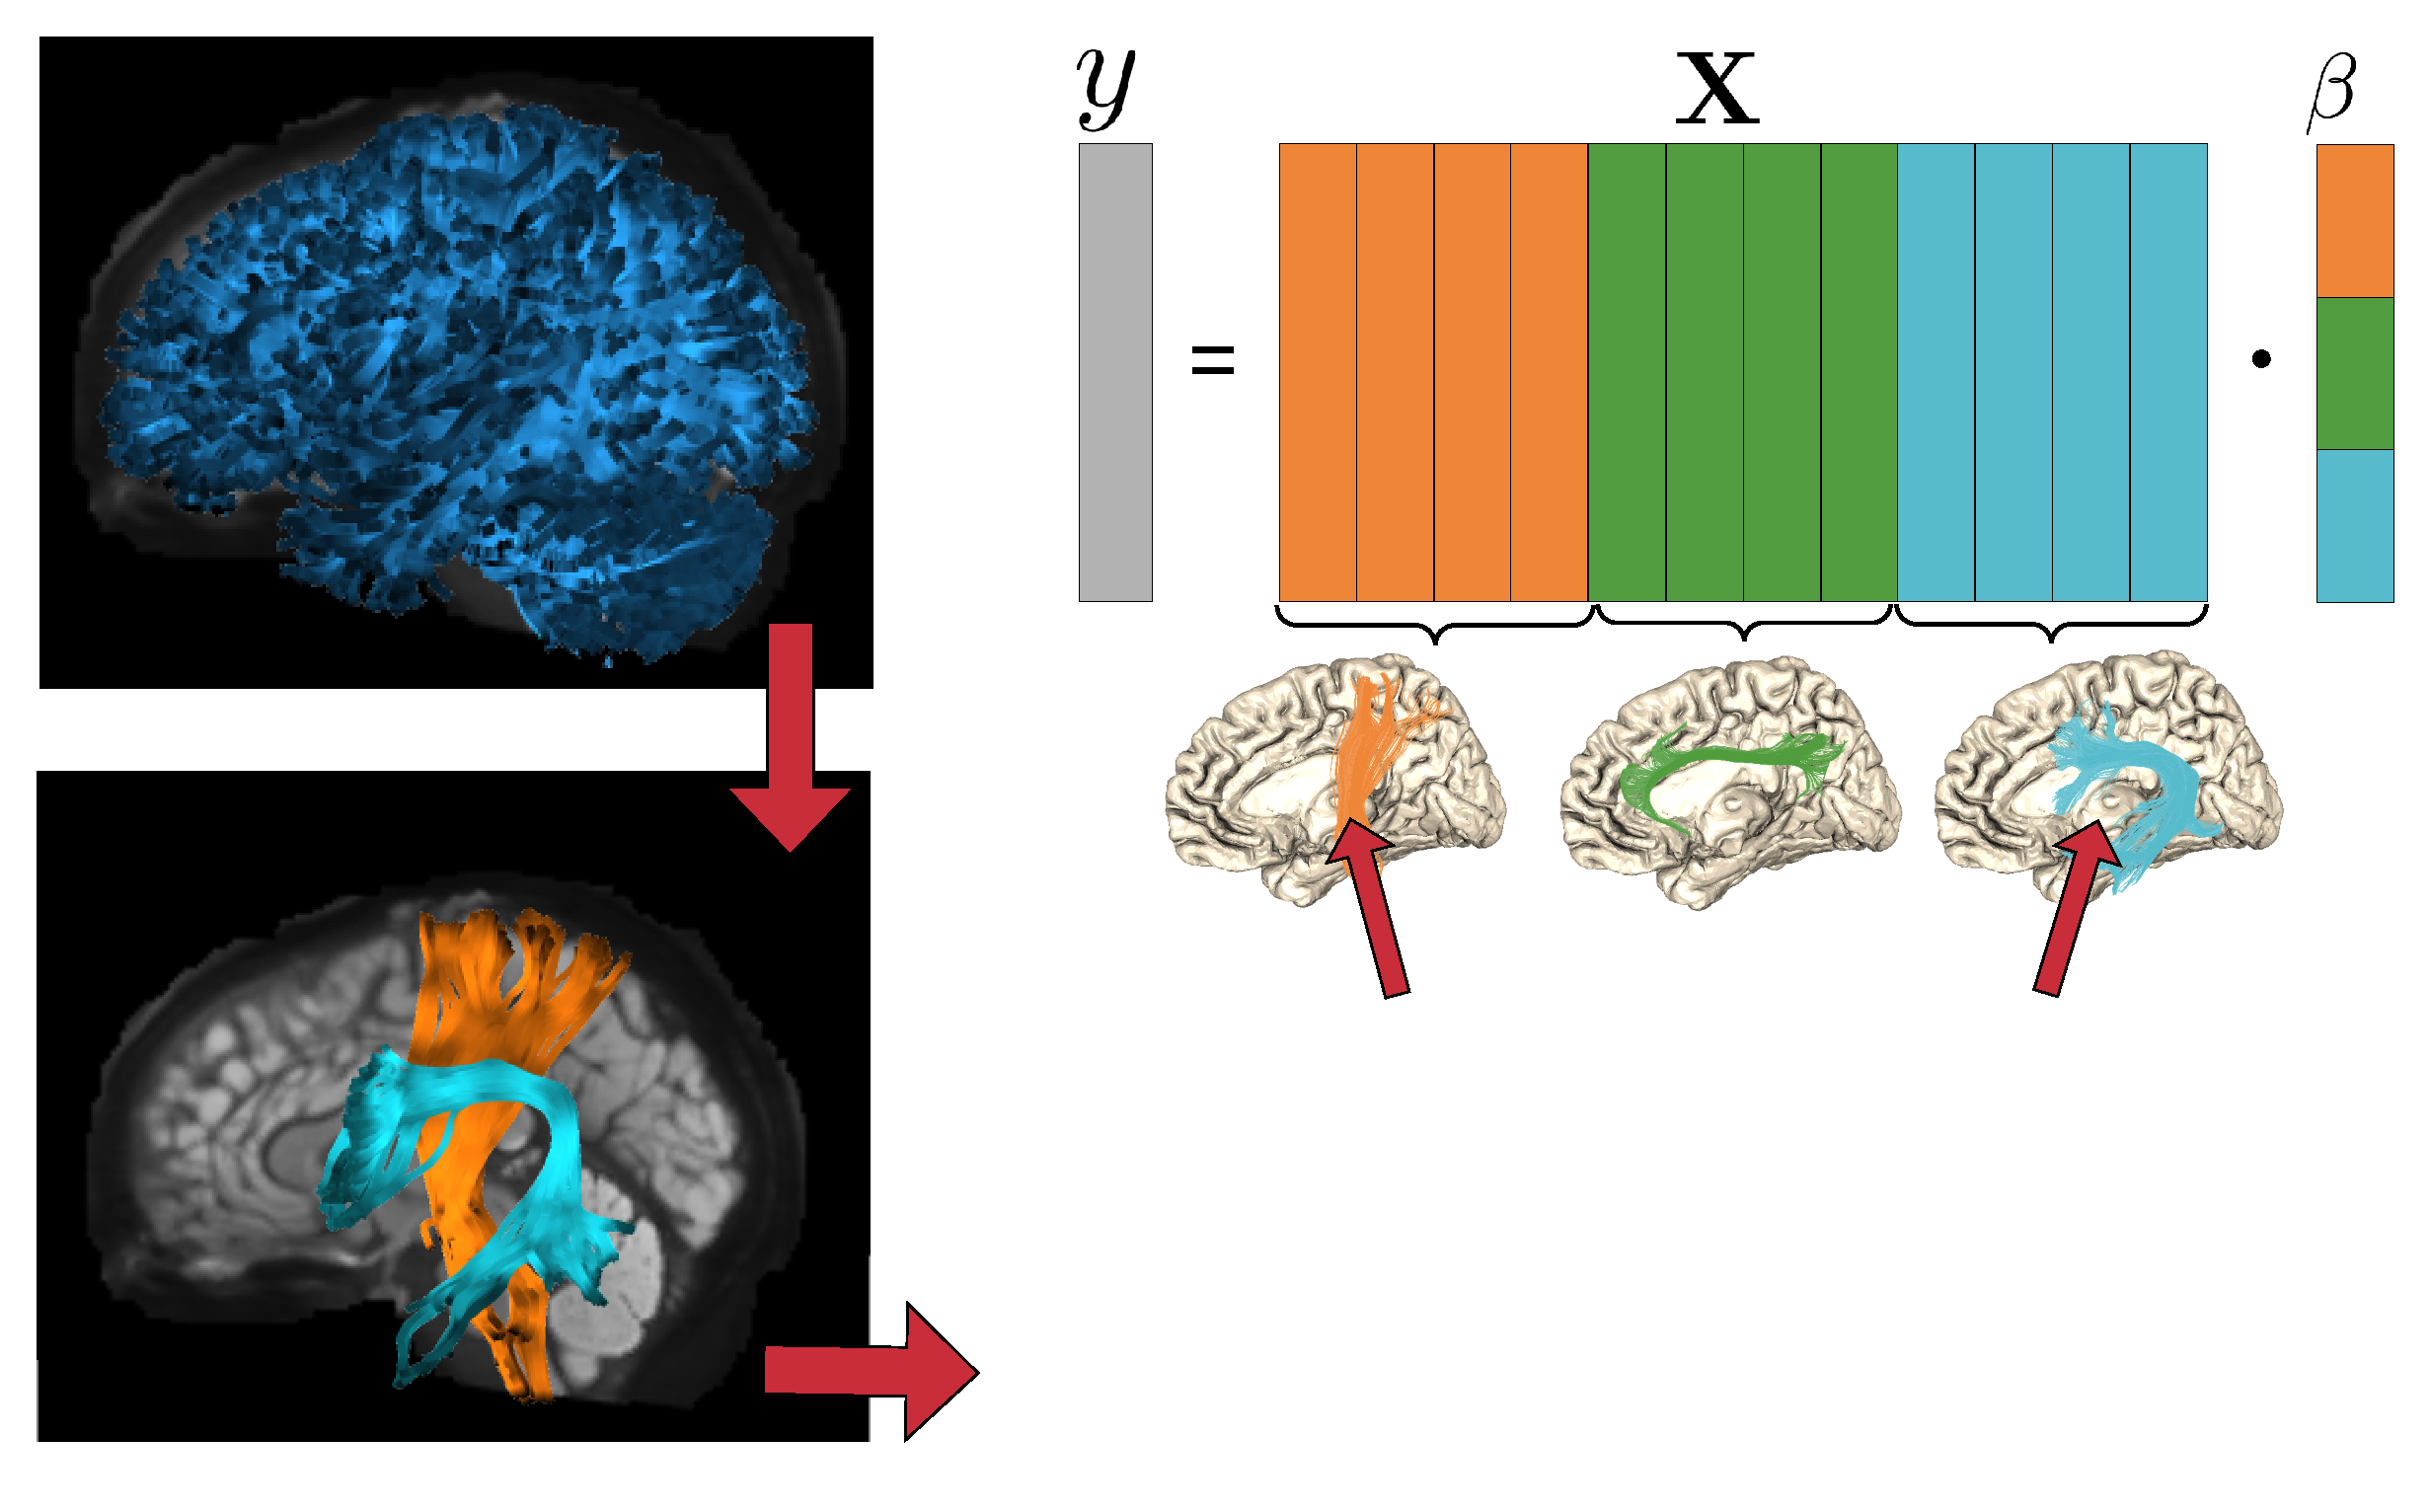
\includegraphics[width=0.98\columnwidth]{methods-brains.pdf}
    }
    \vspace{-9.75cm}
    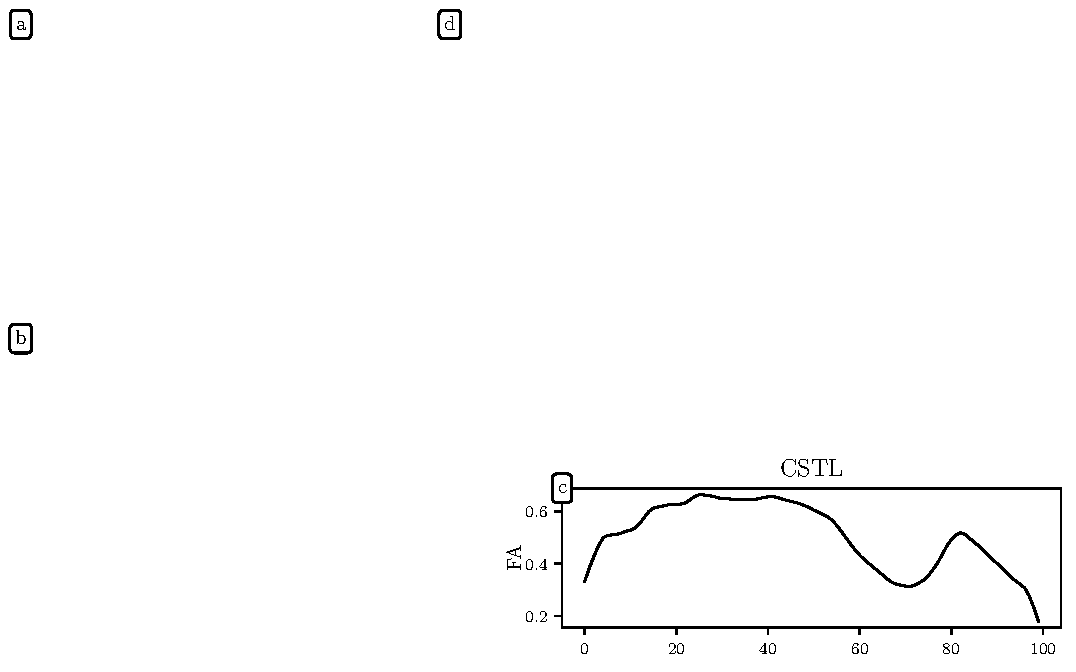
\includegraphics[width=\columnwidth]{method-quad.pdf}
    {\phantomsubcaption\label{fig:methods:tractogram}}
    {\phantomsubcaption\label{fig:methods:cst}}
    {\phantomsubcaption\label{fig:methods:tract-profile}}
    {\phantomsubcaption\label{fig:methods:group-structure}}
    \caption{{\bf Tractometry data flow}
        \label{fig:methods}
        {\bf (a)} Whole brain tractography generates streamlines approximating
        the trajectories of white matter connections.
        {\bf (b)} Tractometry classifies these streamlines into anatomical bundles.
        In this case, we show the left corticospinal tract (CSTL) over a mid-saggital
        anatomical slice.
        {\bf (c)} Tractometry further extracts bundle profiles,
        quantifications of various diffusion metrics along the length of the
        fiber bundle. Here, we show one subject's fractional anisotropy (FA)
        profile for CSTL.
        {\bf (d)} the phenotypical target data and tractometric features can
        be organized into a linear model, $\hat{y} = \mathbf{X}
        \hat{\beta}$. The feature matrix $\mathbf{X}$ is color-coded
        to reveal a natural group structure: the left (orange) group
        contains $k$ features from the CSTL, the middle (green) group
        contains $k$ features from the left cingulum cingulate (CGCL),
        and the right (blue) group
        contains $k$ features from the left arcuate (ARCL). The coefficients in
        $\hat{\beta}$ follow the same natural grouping.
        % Cross-validation:
        % we evaluate model quality using a nested $k$-fold cross validation
        % scheme. At level-0, the input data is decomposed into $k$
        % shuffled groups and optimal hyperparameters are found for the level-0
        % training set.
        % To avoid overfitting, the optimal hyperparameters are themselves
        % evaluated using a cross-validation scheme taking place
        % at level-1 of the decomposition, where each
        % level-0 training set is further decomposed into five shuffled
        % groups. For the ALS and WH data, $k=10$, while for the HBN and
        % Cam-CAN data, $k=5$.
    }
\end{figure}

\todo[inline]{The introduction section should be shortened for Nature methods
I think.}

Non-invasive methods for measuring human brain structure and function have
revolutionized our understanding of brain function. These measurements
have demonstrated that interactions between networks of brain regions give rise
to coordinated information processing and to the complex adaptive behavior that
characterizes human cognition. Diffusion-weighted Magnetic Resonance Imaging
(dMRI) provides a unique view into the physical properties of the connections
that comprise these networks, by sensitizing the measurement to the directional
diffusion of water in each voxel \cite{wandell2016clarifying}.
% While the measurements are usually conducted
% with voxels at the millimeter scale, water molecules within each voxel
% diffuse with characteristic lengths at the micrometer scale, providing
% aggregate information about the physical structure of the white matter,
% including the density of axons and distribution of fiber
% orientations within each voxel \cite{wandell2016clarifying}. Even though
% metrics derived from diffusion measurements are ambiguous in terms
% of their underlying biological interpretation \cite{Jones2013-xv},
% analyzing the variance in these properties has proven useful in
% characterizing individual differences in cognitive function,
% characterizing differences between populations and detecting brain
% abnormalities associated with disease \cite{Thomason2011-qn}.
Methods for computational tract-tracing from diffusion MRI, or tractography,
combine the estimates of fiber orientations in each voxel to form streamlines
that traverse the volume of the white matter~\cite{Conturo1999-je,
Mori2002-qi}. A variety of methods can be used to delineate the
trajectory of major neural pathways among these
streamlines~\cite{yeatman2012tract}.
% These methods have been under increased scrutiny and
% several lines of investigation have raised critiques of their validity
% \cite{Maier-Hein2017-vb, Thomas2014-ki}. On the other hand, there
% have been efforts to shore up the inferences made with these methods
% \cite{Pestilli2014NatMeth, Takemura2016-sh, Smith2013-nc, Smith2015-cx,
% Smith2015-zt, Rheault2018-wk}. Importantly, though discovering novel
% tracts requires extraordinary evidence, and delineating
% the exact cortical termination of the streamlines in the gray matter
% is still prone to error, there is little dispute that tractography
% can accurately define the location of several major white matter
% tracts that are known to exist within the core of the white matter
% \cite{Maier-Hein2017-vb, Catani2002-vu}.
\emph{Tractometry} uses the results of tractography and models
of tissue biophysics based on the patterns of diffusion in each measurement
voxel to assess the physical properties of the white matter along specific
pathways~\cite{Bells2011-cf}.
%Though there are several different available implementations of this overall
%idea, the principles are similar \cite{yeatman2012tract, Yendiki2011-ay,
%Wassermann2016-iv, ODonnell2009-uu}: tractometry begins by delineating
% the parts of the white matter that belong to different major ``tracts''
% (i.e. anatomical or functional groups of white matter fibers), such as
% the corticospinal tract or arcuate fasciculus, assigning tractography
% generated streamlines to ``bundles,'' which approximate the anatomical
% tracts, and sampling biophysical properties, such as fractional
% anisotropy (FA) or mean diffusivity (MD), along the length of these bundles.
% the parts of the white matter that belong to different major tracts
% (i.e. anatomical or functional groups of white matter fibers), such as
% the corticospinal tract or arcuate fasciculus, assigning tractography
% generated streamlines to ``bundles,'' which approximate the anatomical
% tracts, and sampling biophysical properties (such as fractional
% anisotropy or mean diffusivity) along the length of these bundles.
In some previous tractometry-based studies, tissue properties along the
length of each tract were summarized by taking the mean along each
bundle, but there is a large body of evidence showing that there is
systematic variability in the values of diffusion metrics along the
trajectory of each bundle. This justifies retaining the individual
samples along the length of each bundle \cite{yeatman2012tract,
colby2012, ODonnell2009-uu}. While this retains important information
about each individual's white matter, it also presents statistical
challenges due to the dimensionality of the data. In past work,
comparisons between groups or across individuals were done
independently at each node of each bundle, for each one of the
diffusion metrics available at that point. This approach is exhaustive, but
statistical power is compromised by a multiple comparison problem
\cite{colby2012, Nichols2002-zu, Nichols2003-yy}. An alternative that
circumvents the multiple comparison problem is to select just a few
tracts to compare in each individual, or even focusing on particular
segments of these tracts based on \emph{a priori} hypotheses. This
approach is appropriate when the biological basis of the process
of interest is relatively well understood (for a recent example, see
\cite{huber2018rapid}). Sometimes, these approaches are combined: a
bundle is selected based on \emph{a priori} knowledge, and all the data
in the bundle of interest are used together to fit a model that can
predict differences between individuals \cite{dayan2016profilometry}.

% Different approaches can be taken to resolving this challenge. For
% example, Colby and colleagues \cite{colby2012} used a non-parametric
% resmapling approach to
% correct for family-wise error across the different possible comparisons
% \cite{Nichols2002-zu, Nichols2003-yy}.
% Based on tractometry, researchers may choose to compare different individuals
% to each other. This is usually done according to one of the following
% approaches:
% \begin{enumerate}
% \item Mass univariate approaches: In this approach


% \item Region of interest(ROI)-based approaches:
% An alternative that
% circumvents the multiple comparison problem is to select just a few
% tracts to compare in each individual, or even focusing on particular
% segments of these tracts based on \emph{a priori} hypotheses. This
% approach is very powerful when the biological basis of the process
% of interest is relatively well understood (for a recent example, see
% \cite{huber2018rapid}).

% \item ROI-based selection, followed by multivariate analysis: Here,
% an ROI is selected based on \emph{a priori} knowledge, and all the
% nodes or voxels in the ROI are used together to fit a model that can
% predict differences between individuals. An example of that is the
% ``profilometry'' framework, in which different diffusion metrics
% from a single tract are combined together to provide input to a
% multivariate analysis of covariance, and linear discriminant analysis
% \cite{dayan2016profilometry}.

%\end{enumerate}

The present work aims to balance predictive
accuracy with descriptive power \cite{Murdoch2019-ax, Breiman2001-uz}
by capitalizing on all of the data across all bundles, while also retaining and
elucidating spatial information about the locations that are most informative
for discriminative performance. To do so, we use a linear modeling approach,
which aims to redict phenotypical variance in a group of subjects, based on a
linear combination of the features estimated with tractometry.

% Generally speaking, analysis methods should balance predictive
% accuracy with descriptive power \cite{Murdoch2019-ax, Breiman2001-uz}.
% Accordingly, tractometry analysis should simultaneously capitalize on
% all the data across all tracts to make the best possible prediction,
% while also retaining and elucidating spatial information about the
% locations that are most informative for a prediction. In the present
% work, we developed a novel framework for analysis of tractometry that
% simultaneously selects the features for analysis, and fits a model
% to these features. We use a linear modeling approach, which aims to
% predict phenotypical variance in a group of subjects, based on a linear
% combination of the features estimated with tractometry.

Using this approach, we first need to deal with the large and
asymmetric dimensionality of the data: tractometry data usually has
many more features (i.e., number of measurements per individual) than
samples (number of subjects), which makes inferences from the data
about phenotypical differences between individuals ill-posed. This
regime is the target of several statistical learning techniques, and
is often solved by various forms of regularization.

% For example, Tikhonov regularization shrinks the solution such that the sum of
% squared contributions from the individual features are minimized
% \cite{Hoerl2000-ij}. Another solution to the problem is provided by
% the

The Lasso algorithm minimizes the sum of the absolute values of
contributions of each feature \cite{Tibshirani1996-qs}. This
tends to shrink to zero the contributions of many of the features,
providing results that are both accurate and interpretable. When
additional structure is available in the organization of the data,
regularization algorithms can take advantage of this structure. For
example, if the features lend themselves to a natural division into
different groups, the group lasso (GL) can be used to select groups
of features, rather than individual features \cite{Yuan2006-ky}.
The Sparse Group Lasso (SGL) elaborates on this idea by providing
control both of group sparsity, as well as overall sparsity of the
solutions \cite{simon2013sgl}. Because the features measured with
tractomery lend themselves to grouping based on the tracts from which
each measurement is taken, GL and SGL provide useful tools
for linear model fitting in problems of this form. Here we, first,
develop an implementation of SGL that is well suited to the analysis of
tractometry data and, second, demonstrate the power and flexibility of
this approach by applying it to both classification
and continuous prediction problems.
